\section{\vita: Challenges}
\label{sec:example}
\todo{Borrow the Teddy usecase as example. Drop data mangement challenges like C3 and C5. Drop D3 and D5.}

\saj{SAJ: my takeaways from the CHI 2020 paper:}
\todo{\textbf{Setup}. Participants stated they often downloaded data outside of the notebook from various data sources since interfacing with them programmatically was too much hassle. Not only that, but notebooks often crash with large data sets (possibly due to the notebooks running in a web browser). Once the data is loaded, it then has to be cleaned, which participants complained is a repetitive and time consuming task that involves copying and pasting code from their personal "library" of commonly used functions.}

\saj{This maps to having a the Data View to get immediate feedback in pre-processing operations, providing a operations menu to avoid copy-pasting repeated code. Also solves the problem of discoverability. If there's no existing operations, users can define UDFs to reuse later.}

\todo{\textbf{Explore and analyze.} Modeling and visualizing data are common tasks but can become frustrating. For example, we observed one participant tweak the parameters of a plot more than 20 times in less than 5 minutes. Moreover, building models break the quick and iterative workflow of notebooks since it can take several minutes or longer to finish.}

\saj{we don't solve the model building problem or the interactivity issue. but sampling or filtering is a solution to work on a small data subset and do quick and dirty analysis. Exploration is a big plus in our system with added bonus of dynamic coordination.}.

\todo{\textbf{Manage code.} Notebooks do not have all of the features of an IDE, like integrated documentation or sophisticated autocomplete, so participants often switch back and forth between an IDE (e.g., VS Code) and their notebook. One participant we observed kept both windows side-by-side and copy and pasted code between the two windows rapidly as they worked. Another major pain point is managing package dependencies. Participants also indicated that they develop their own processes for debugging and testing, and some expressed irritation with the lack of tool support.}

\saj{We have autocomplete feature in the input field of the Code Editor. However, debugging errors is a weakness. The strength is any dataframe transformation becomes immediately visible in the Data View. A nice to have will be having the ability to view metadata. Users can immdeidately relate visual representation with raw data---not even available in IDEs.}

\todo{textbf{Reliability.} It is not uncommon for a notebook's kernel to crash in the middle of an operation, which may leave the notebook or data in an inconsistent state without proper feedback to the user. Participants commented that they find it easier to just restart and run the entire notebook again with hopes that it doesn't crash. Additionally, notebooks have limitations when it comes to big data, which requires users to move to a different tool set (e.g., Java or Python scripts).}

\saj{we have same issues. But I feel like this is challenge of any existing tool---fault tolerance.}

\todo{\textbf{Archival.} Participants expressed much difficulty with using version control systems for notebooks. For example, the outputs are saved in the notebooks along with metadata, which will always indicate changes to the version control system. Searching and finding information from previous notebooks is also an unsolved challenge.}

\saj{was part of our leam vision but we don't have that yet. But our system is set up to support that. By managing task queues and view caches we can measure the delta of states of data and code per instruction and save those delta for lineage or provenance.}

\todo{\textbf{Security.} Participants were concerned about sensitive data that may need to be masked from other users while still allowing them to execute the notebook. Notebooks also don't support restrictions such as read-only or run-only, thus requiring external tools to enforce access.
Share and collaborate. While it is easy to share the notebook file, it is often not easy to share the data. For example, the data may require access to a database. Participants said that they often need to create documentation to explain how to install and setup any necessary dependencies to run a notebook. Furthermore, there is missing support for sharing the notebook results with others, especially non-technical users, for the purposes of reports or presentations.}

\saj{out of our scope}

\todo{\textbf{Reproduce and reuse.} Due to the dependency issues and environment settings, it is unlikely that a notebook will work out of the box. Reusing even small portions of a notebook is difficult due to package dependencies and even dependencies on other cells within the notebook.
Notebooks as products. If a large data set is used, as one might expect in production, then the notebook will lose the interactivity while it is executing. Also, notebooks encourage "quick and dirty" code that may require rewriting before it is production quality. For example, participants indicated that notebooks are not always designed to be executed top to bottom, which will require additional work to fix the execution order for a standalone artifact.}

\saj{we support code reuse as new operations are continuously added and UDFs can be preserved. the environment setting is also a pain point that we don't address. but I can imagine adding any new import as part of the requirement.txt file in the backend build directory and export that setting file. Users can just use the exported settings file in another project. }


\stitle{Motivating Example.} 
Ada, a data scientist in the e-commerce department of a retail business, has been tasked to analyze customer reviews of products purchased from their website. Ada would like to capture the underlying topics by performing topic modeling and clustering to characterize the review corpus better. Figure~\ref{fig:workflow} captures the use-case which involves---(a) preprocessing the data (\emph{clean}), creating feature vectors from the text reviews (\emph{featurize}), creating topic vectors from the corpus (\emph{topic modeling}), clustering reviews into topics (\emph{cluster assignment}), and finally, visualizing the clusters by projecting the topics vectors to lower dimensions (2D) using feature transformation techniques such as PCA (\emph{visualize}). In practice, the workflow may be non-linear, and each step may require multiple passes and different tools. In the process, visualizations are useful not only for exploratory analysis or final presentation but also for every other step---\vita workflows resemble the \emph{read-eval-print loop} (REPL) approach where users perform incremental operations on data and examine intermediate results. We now characterize the challenges of the existing \vita  workflows in the context of this use-case as follows:

\emtitle{C1. Overhead due to data and tasks heterogeneity.} As mentioned in Section~\ref{sec:intro}, data scientists lack tools 
that support different \vita operations and workflows within an integrated environment.
For example, to define the data cleaning rules, Ada first visually inspects the data using tools like spreadsheets. Next, they execute those rules in a computational notebook, \eg Jupyter. Upon inspecting the data in the spreadsheet, Ada may revise the rules in the notebook. To visualize top-ranked words after the featurization step (\eg a bar chart of words ranked by their TF-IDF scores), they need to either use dedicated visualization tools or write scripts in the notebook. Therefore, even completing simple tasks may require accessing different tools, which can be cumbersome user experience due to, for example, the logistical and cognitive overhead of context switching.
 
\emtitle{C2. Tension between interactivity and expressivity.}  \vita necessitates coordination among different views (\eg between visualization and raw data).  The high dimensional text data can be difficult to interpret and users often map different facets of the data to visualizations for better interpretability. 
However, without coordination between perceptual components and the data space, understanding the relations between the facets of the same entities on demand can be challenging. 
For example, say Ada wants to inspect which reviews contain a top-word shown in a  bar chart (generated after featurization). However, visualizations in notebooks or visualization tools are decoupled from the data. As a result, Ada has to either open and then filter the data in a spreadsheet, or programmatically filter the data from the notebook to inspect the relevant reviews. Therefore, the lack of coordination impacts both workflow continuity and the user's ability to explore data effectively.
 
\begin{figure}[tbp] 
%  \vspace{-10pt}
  \centering
  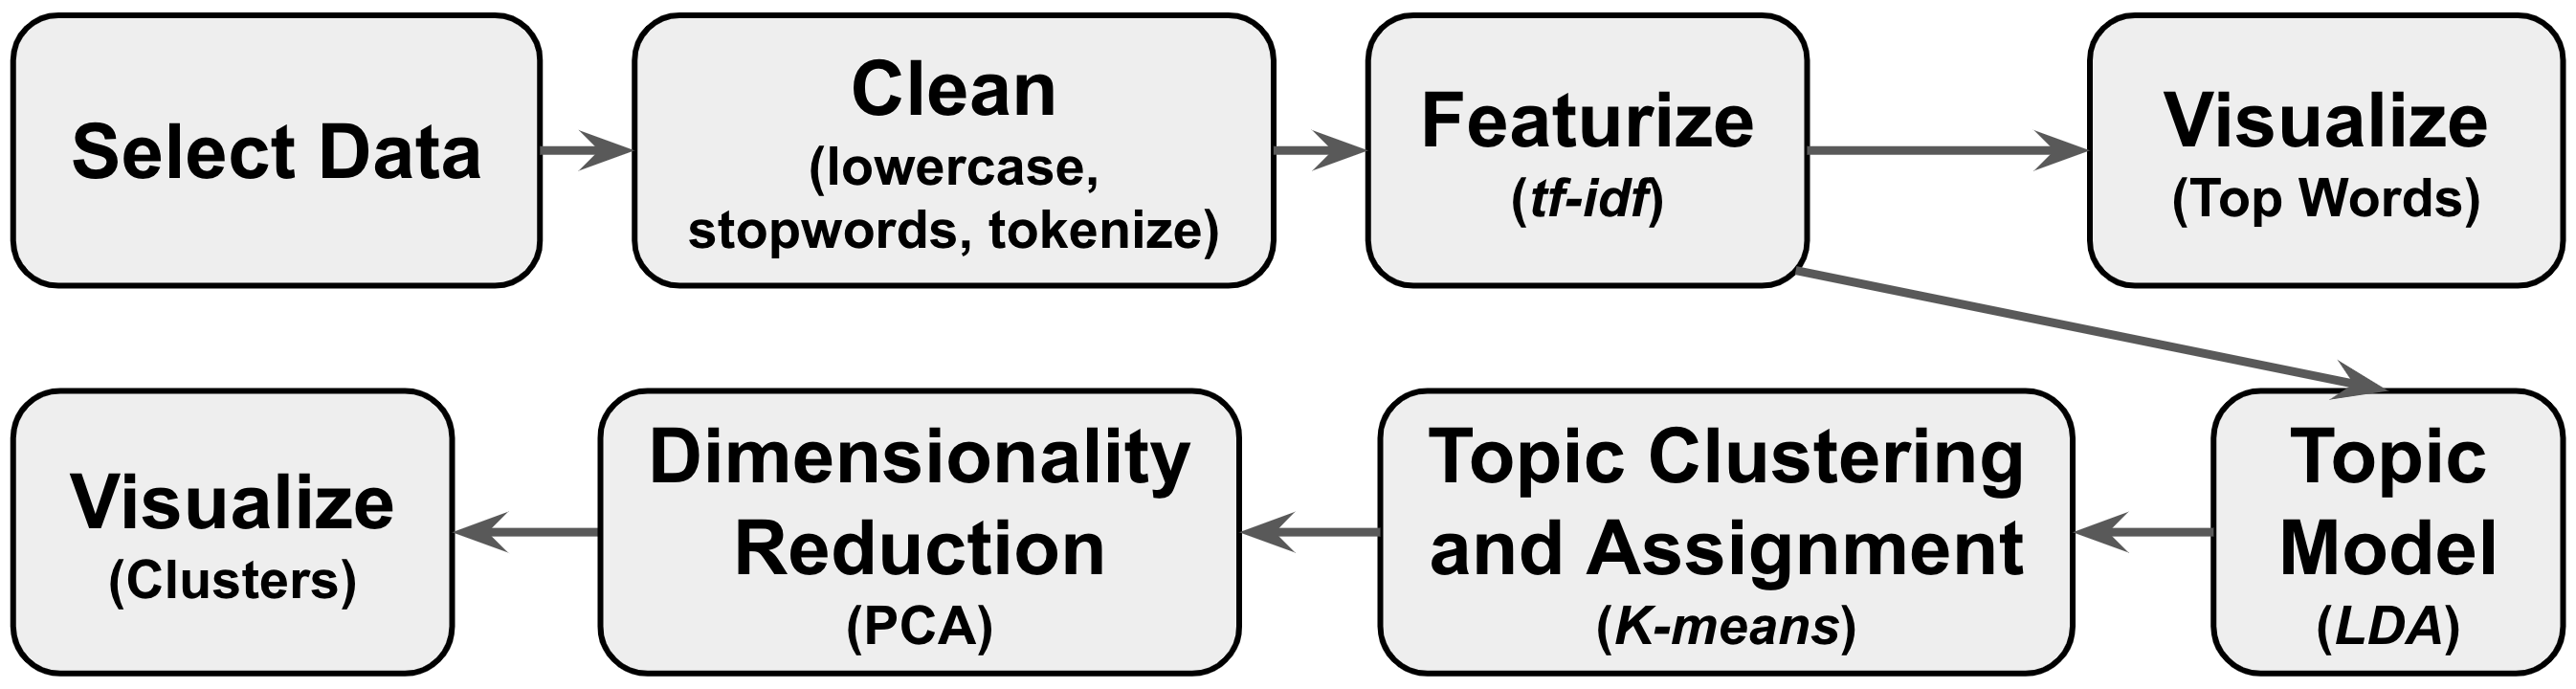
\includegraphics[width=\linewidth]{figures/workflow.png}
  \caption{\small An example \vita workflow for topic exploration. Even this basic workflow contains a diverse set of tasks. Interactive visualizations are useful across multiple stages in the workflow.\label{fig:workflow}} 
%   \vspace{-20pt}
\end{figure}

% \emtitle{C3. Data types and workflow diversity.} \vita workflows deal with heterogeneous data (\eg text, visualizations) and workflows (\eg in use-cases like text summarization, sentiment analysis). While there are a number of \vita tools for specific workflows~\cite{liu2018bridging}, more often than not these tools use a stack of independent solutions for data storage and
% processing glued together by scripting languages like Python and R.
% These bespoke solutions typically don’t support direct data manipulation and interactive visual coordination. As a result, users are often forced to develop new and heavily customized systems on top of these solutions.

\emtitle{C3. Arduous workflow authoring.} 
\vita workflows contain a variety of operations, \eg cleaning, featurization, interactive visualization, classification. Similar to relational~\cite{codd} or data visualization algebra~\cite{satyanarayan2016vega}, \vita operations with similar objectives can be grouped into high-level categories. Moreover, operations in different categories can be combined to compose new operation pipelines. For example, cleaning and featurization can be combined into a preprocessing pipeline. As existing systems lack any formalization of the operations and their application, the onus is on the user to design the optimal analytics workflow for different use-cases.

% \emtitle{C5. \vita Session management.} As demonstrated in the usage example, \vita workflows warrant the trial-and-error style  iterative approach---users often need to reproduce previous steps of the workflow, make updates, and rerun the subsequent steps. 
% Therefore, ensuring reproducibility of  \vita sessions requires management of dataset versions produced by various operations, the operation logs, and different states of and interactions on the visual representations of the data. 
% Prior work from the data management community focused on versioning structured datasets~\cite{huang2017orpheusdb}, versioning code for debugging workflows~\cite{brachmannbyour,miao2016provdb} and managing deep learning models~\cite{miao2016modelhub}.
% However, these systems lack support for versioning an end-to-end \vita workflow involving heterogeneous data types and user interactions spanning multiple views. 

